\documentclass[a4paper,12pt]{article}
\usepackage[chinese, provide=*]{babel}
\usepackage{starfont} % 添加天文符号
\usepackage{amsmath, amsthm}
\usepackage{datetime}
\usepackage{framed}
\usepackage{enumitem}
\usepackage{fancyref}
\usepackage{wrapfig}
\usepackage{pifont}
\usepackage{appendix}
\usepackage{caption}
\usepackage{xcolor}
\usepackage[stable]{footmisc}
\usepackage{multicol}
\usepackage{csquotes}

\usepackage{amsthm}
\usepackage{amssymb}
\usepackage{amsfonts}
\usepackage{amsmath}
\usepackage{mathtools}

\usepackage{tikz}
\usepackage{pgf}
\usepgflibrary{fpu}
\usepackage{qtree}
\usetikzlibrary{angles,fit,arrows,calc,math,intersections,through,backgrounds}
\usepackage{pgfplots}
\usepackage{tkz-euclide}

\usepackage{listings}
\lstset{
  basicstyle=\itshape,
  xleftmargin=3em,
  literate={->}{$\rightarrow$}{2}
           {α}{$\alpha$}{1}
           {δ}{$\delta$}{1}
}


\usepackage{csquotes}
\renewcommand{\mkbegdispquote}[2]{\itshape}

\newdateformat{nianyueri}{ \THEYEAR 年 \THEMONTH 月 \THEDAY 日 }

\usepackage{xstring}
\usepackage{catchfile}
\CatchFileDef{\HEAD}{../.git/refs/heads/master}{}
\newcommand{\gitrevision}{%
  \StrLeft{\HEAD}{7}%
}

\usepackage{data/quiver}
\usepackage{data/circledsteps}
\usepackage[top=1in,bottom=1in,left=1in,right=1in]{geometry} % 用于设置页面布局
\usepackage{xeCJK} % 用于使用本地字体
\usepackage[super, square, sort&compress]{natbib} % 处理参考文献
\usepackage{titlesec, titletoc} % 设置章节标题及页眉页脚
%\usepackage{xCJKnumb} % 中英文数字转换
\usepackage{amssymb}
\usepackage{amsmath} % 在公式中用\text{文本}输入中文
\usepackage{diagbox}
\usepackage{multirow} % 表格中使用多行
\usepackage{booktabs} % 表格中使用\toprule等命令
\usepackage{rotating} % 使用sidewaystable环境旋转表格
\usepackage{tabularx}
\usepackage{graphicx} % 处理图片
\usepackage{footnote} % 增强的脚注功能,可添加表格脚注
\usepackage{threeparttable} % 添加真正的表格脚注,示例见README
\usepackage{hyperref} % 添加pdf书签

\usepackage{tikz}
\usetikzlibrary{shapes,arrows,shadows}

% 字体设置
\setmainfont{Times New Roman}
\setsansfont[Scale=MatchLowercase,Mapping=tex-text]{PT Sans}
\setmonofont[Scale=MatchLowercase]{PT Mono}
\setCJKmainfont[ItalicFont={Kaiti SC}, BoldFont={Heiti SC}]{Songti SC}
\setCJKsansfont{Heiti SC}
\setCJKmonofont{Songti SC}
% \setCJKmainfont[BoldFont={FZXiaoBiaoSong-B05S}]{Songti SC}
% \setCJKfamilyfont{kai}[BoldFont=Heiti SC]{Kaiti SC}
% \setCJKfamilyfont{song}[BoldFont=Heiti SC]{Songti SC}
% \setCJKfamilyfont{hei}[BoldFont=Heiti SC]{Heiti SC}
% \setCJKfamilyfont{fsong}[BoldFont=Heiti SC]{Songti SC}
% \newcommand{\kai}[1]{{\CJKfamily{kai}#1}}
% \newcommand{\hei}[1]{{\CJKfamily{hei}#1}}
% \setromanfont[Mapping=tex-text]{TeXGyrePagella}
% \setsansfont[Scale=MatchLowercase,Mapping=tex-text]{TeXGyrePagella}
% \setmonofont[Scale=MatchLowercase]{Courier New}
%%设置常用中文字号,方便调用
\newcommand{\erhao}{\fontsize{22pt}{\baselineskip}\selectfont}
\newcommand{\xiaoerhao}{\fontsize{18pt}{\baselineskip}\selectfont}
\newcommand{\sanhao}{\fontsize{16pt}{\baselineskip}\selectfont}
\newcommand{\xiaosanhao}{\fontsize{15pt}{\baselineskip}\selectfont}
\newcommand{\sihao}{\fontsize{14pt}{\baselineskip}\selectfont}
\newcommand{\xiaosihao}{\fontsize{12pt}{\baselineskip}\selectfont}
\newcommand{\wuhao}{\fontsize{10.5pt}{\baselineskip}\selectfont}
\newcommand{\xiaowuhao}{\fontsize{9pt}{\baselineskip}\selectfont}
\newcommand{\liuhao}{\fontsize{7.5pt}{\baselineskip}\selectfont}

% 章节标题显示方式及页眉页脚设置
% \item xCJKnumb是自己额外安装的包
% \item titleformat命令定义标题的形式
% \item titlespacing定义标题距左、上、下的距离
\titleformat{\section}{\raggedright\large\bfseries}{\thesection}{1em}{}
\titleformat{\subsection}{\raggedright\normalsize\bfseries}{\thesubsection}{1em}{}
\titlespacing{\section}{0pt}{*0}{*2}
\titlespacing{\subsection}{0pt}{*0}{*1}
% 由于默认的2em缩进不够,所以我手动调整了,但是在windows下似乎2.2就差不多了,或者是article中没有这个问题
\setlength{\parindent}{2.2em}

% 设置表格标题前后间距
\setlength{\abovecaptionskip}{0pt}
\setlength{\belowcaptionskip}{0pt}


\renewcommand{\refname}{\bfseries{参~考~文~献}} %将Reference改为参考文献(用于 article)
% \renewcommand{\bibname}{参~考~文~献} %将bibiography改为参考文献(用于 book)
\renewcommand{\baselinestretch}{1.38} %设置行间距
\renewcommand{\figurename}{\small\ttfamily 图}
\renewcommand{\tablename}{\small\ttfamily 表}


\usepackage{stmaryrd}
\usepackage{mathtools}
\usepackage{wasysym}
\usepackage{textcomp}
\usepackage{subfiles}

\newtheorem{problem}{问题}
\numberwithin{problem}{section}
\newtheorem{definition}{定义}
\numberwithin{definition}{section}
\newtheorem{lemma}{引理}
\numberwithin{lemma}{section}
\newtheorem{proposition}{命题}
\numberwithin{proposition}{section}
\newtheorem{theorem}{定理}
\numberwithin{theorem}{section}
\newtheorem{grammar}{文法}
\numberwithin{grammar}{section}
\newtheorem{program}{程序}
\numberwithin{program}{section}
\newtheorem{convention}{约定}
\numberwithin{convention}{section}
\newtheorem{corollary}{推论}
\numberwithin{corollary}{section}
\renewcommand*{\proofname}{证明}

\xeCJKsetwidth{‘’“”}{1em}

\usepackage[acronym,xindy]{glossaries}
\renewcommand*{\glossaryname}{术~语~列~表}
\makeglossaries

\usepackage[xindy]{imakeidx}
\makeindex

\loadglsentries[main]{glossary}

\title{学习是否超越了图灵计算?}
\date{\nianyueri\today}
\author{苑明理、孙伊}

\begin{document}
\selectlanguage{chinese}

\maketitle
\begin{abstract}
    学习是否超越了图灵计算?本文我们给出这个问题的正反两种观点,并予以辨析。
\end{abstract}

\renewcommand\contentsname{目录}
\setcounter{tocdepth}{2}
\tableofcontents
\newpage

\section{引言}

罗伯特·罗森在《有效过程与自然法则》\cite{Rosen1988EffectivePA}的开篇就陈述了一个宏大科学史的场面。
\begin{displayquote}
现代科学史上最引人注目的思想交汇之一,发生在 1931 年哥德尔关于形式不可判定性原始论文发表
与 1943 年麦卡洛克和皮茨关于神经网络著作发表之间的短短几年间。 在这十二年中,逻辑学、数学、大脑理论和数字计算的可能性
之间建立了基本的相互关系,现在想起来所有这些仍然让人叹为观止。人们当时认为,半个世纪之后的今天也依然认为,这些思想预示着一场根本性的革命,
恰如三个世纪前牛顿所取得的进展一样。
\end{displayquote}

\begin{figure}[ht]
\centering
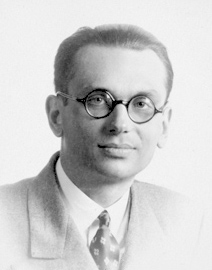
\includegraphics[height=1.5in]{images/kurt_godel.jpg}
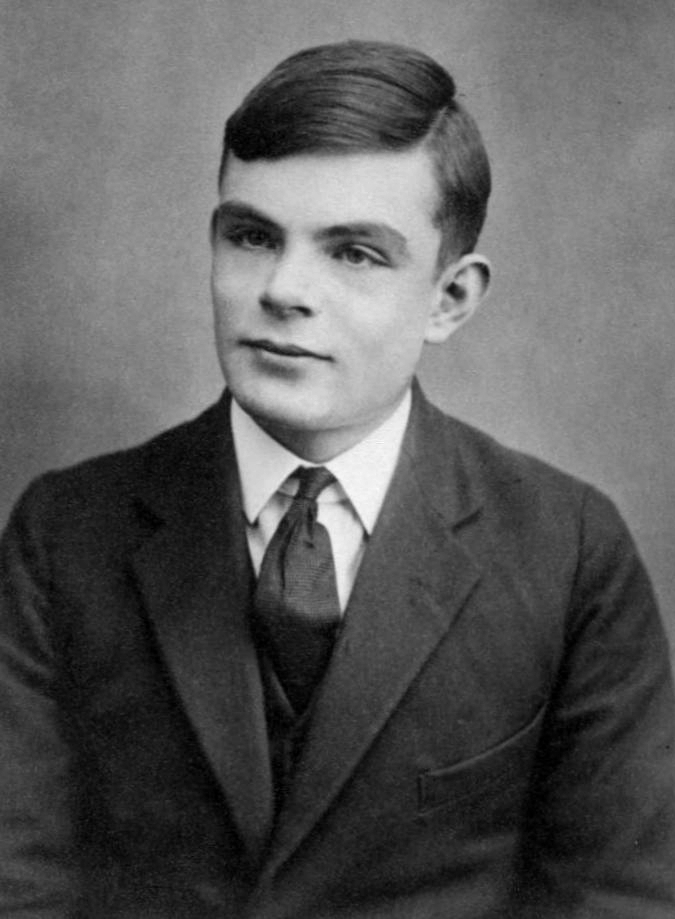
\includegraphics[height=1.5in]{images/alan_turing.jpg}
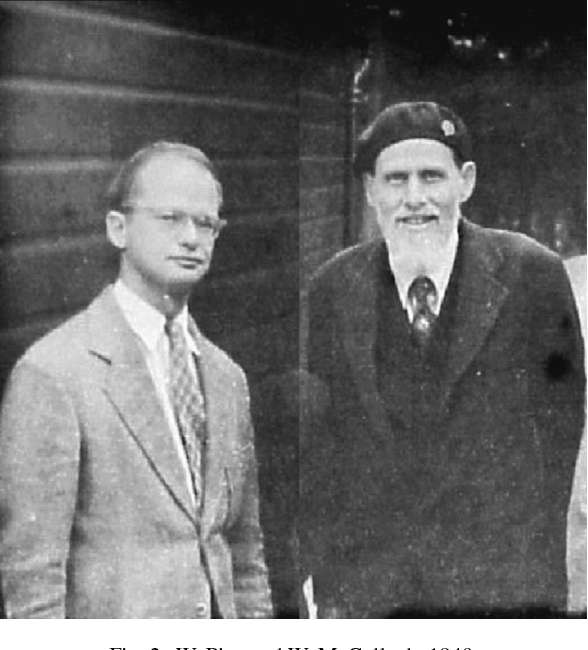
\includegraphics[height=1.5in]{images/pitts_mcculloch_1949.png}
\caption{青年哥德尔;青年图灵;皮茨和麦卡洛克的合照}
\end{figure}

这段恢宏的学科开创历史已经过去了八、九十年,此后人们在逻辑学、计算理论、学习理论、脑科学、深度学习等方面都取得了长足的进展,然而对一些基本问题
人们仍然存有争议,比如:
\begin{itemize}
    \item 图灵-邱奇论题的意义?\cite{Boker2020WhatIT}
    \item 超计算是否存在?\cite{Copeland2004Hypercomputation}
    \item 计算与物理的关系\cite{Copeland2018CTT}
\end{itemize}

很少有人把学习加入到上述讨论之中,在这篇短文里,我们将探讨学习是否是一种超越了图灵计算的问题,并给出正反两种观点的总结。

\section{第一类学习问题}

\subsection{巨石阵的假说}

对今天的考古学家、天文学家来说,建造巨石阵的目的和它设计形式里的含义始终是一个未解之谜;但人们长久以来一直怀疑,巨石阵可以用来进行天文观测
并有它的历法含义,相关的假说从 1740 年斯图克利(Stukeley)开始一直延续至今。霍金斯(Hawkins) 和霍伊尔 (Hoyle)分别在 1963 年和 1966 年
提出了巨石阵内 56 个奥布里洞(Aubrey holes)可以用来定位日月位置并预测日月食的发生。\cite{Herten2018FunctionalPO}

\begin{figure}[ht]
\centering
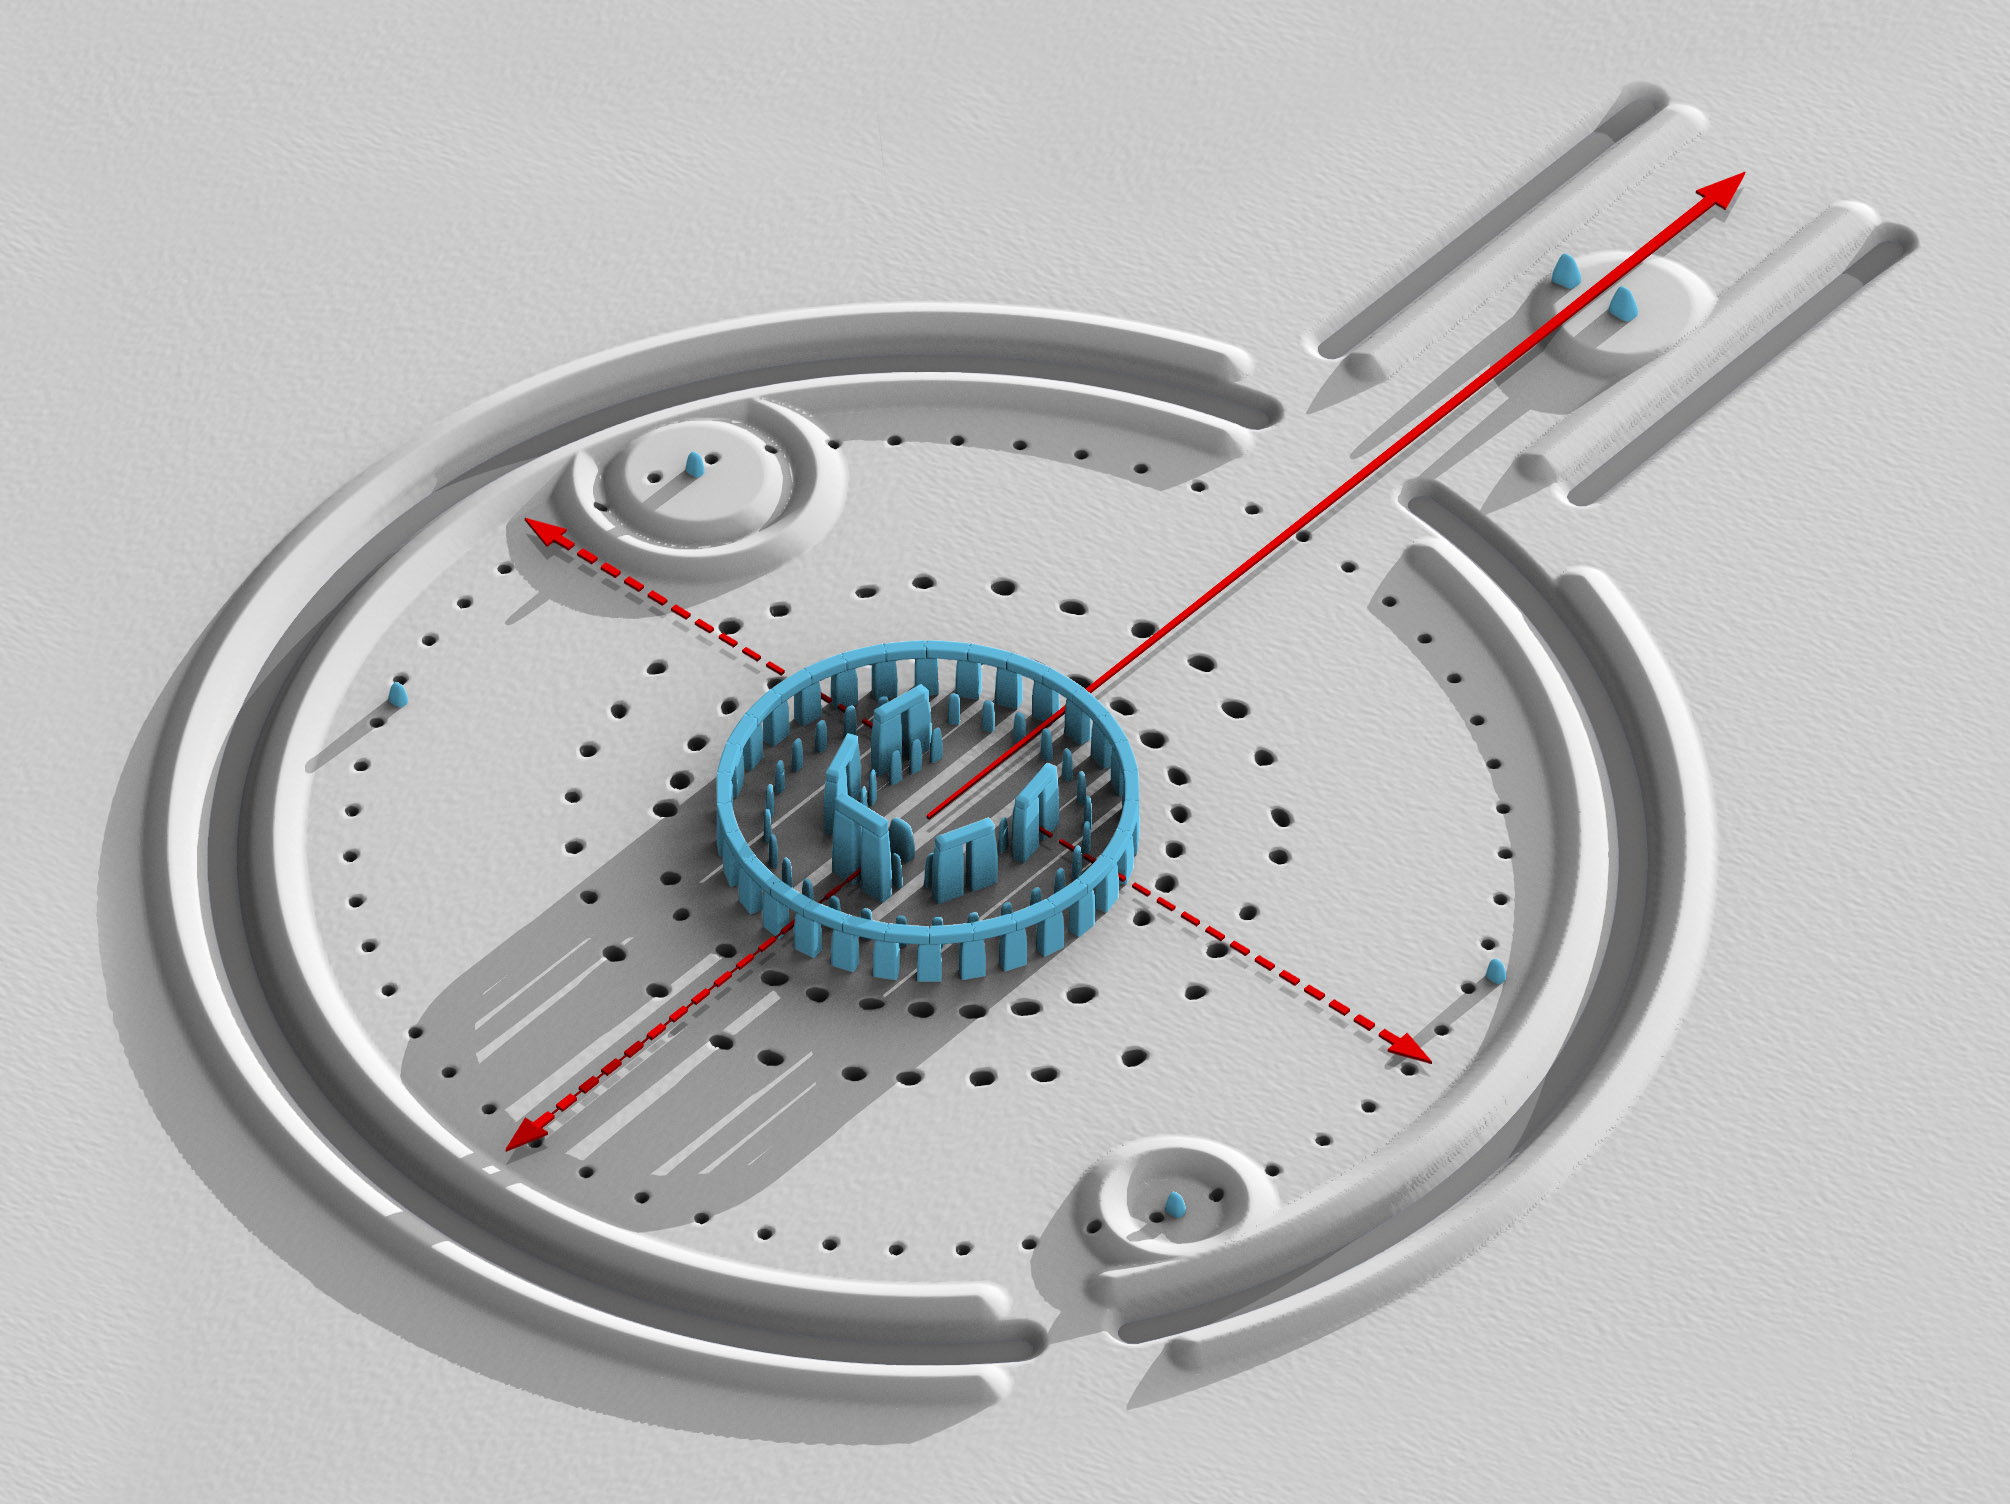
\includegraphics[width=5.0in]{images/Stonehenge_render.jpeg}
\caption{巨石阵全貌的模拟图(来自于维基共享资源计划)}
\end{figure}

假想的预测原理是基于太阳的运动周期(地球的周年运动)、月球的运行周期和沙罗周期的近似表达展开的。可以把沙盘的圆周等分成 56 份,
然后在上面简单地计数来模拟日、地、月的运行,并不断通过观测来校正,这样就可以使整个预报系统长期精确地运行。\cite{beggs2012unifying}

\begin{table}[tbhp]
\centering
\begin{tabular}{|c|c|c|c|}
\hline
天文现象 & 周期 & 近似周期 & 沙盘移动方法 \\
\hline
太阳的运行周期 & 365.26 天 & $ 56 \times \frac{13}{2} $ & 每 13 天移动 2 步 \\
\hline
月球的运行周期 & 27.32 天 & $ 56 \times \frac{1}{2} $  & 每天移动 2 步 \\
\hline
沙罗周期 & 18.61 年 & $ 56 \times \frac{1}{3} $  & 每年移动 3 步 \\
\hline
\end{tabular}
\caption{基于 56 的日食预测原理}
\end{table}

下图是设想中的巨石阵预测方法:在 56 个奥布里洞上插入 4 把旗帜,有两把分别代表日、月,另外两把代表沙罗周期,人们可以据此模拟日月运行和食变。
代表太阳的旗帜,每 13 天逆时针移动 2 个洞;代表月亮的旗帜,每天逆时针移动 2 个洞;代表沙罗周期的两把旗帜,相互在对方的对径点上,每年顺时针移动 3 个洞。
当这些旗帜彼此接近的时候,就有可能发生食变。

\begin{figure}[ht]
\centering
\begin{tikzpicture}[rotate=10]
    \draw (0,0) ellipse (6 and 3);
    \foreach \a in {1,...,56}
    {
        \node (n\a) at ({
            \a * 6.428571428571429
        }:{
            3.0 / sqrt(1 - 0.75 * cos(\a * 6.428571428571429) * cos(\a * 6.428571428571429)))
        }){};
    }
    \foreach \a in {1,...,56}
    {
        \fill (n\a) circle [radius=2pt];
    }
    \foreach \a in {1,...,56}
    {
        \node (o\a) at ({
            \a * 6.428571428571429
        }:{
            4.0 / sqrt(1 - 0.75 * cos(\a * 6.428571428571429) * cos(\a * 6.428571428571429)))
        }){};
    }
    \node[circle, draw] (sun) at ($(n21) + (80:1)$) {\Sun};
    \node[circle, draw] (moon) at ($(n38) + (80:1)$) {\Moon};
    \node[circle, draw] (saros1) at ($(n31) + (80:1)$) {$\sigma$};
    \node[circle, draw] (saros2) at ($(n3) + (80:1)$) {$\sigma$};
    % phases
    \draw[dotted](n56)--(n28);
    \draw[dotted](n14)--(n42);
    \node[dotted, circle, draw] (W) at ($(n56)!0.5!(o56)$) {西};
    \node[dotted, circle, draw] (S) at ($(n14)!0.5!(o14)$) {南};
    \node[dotted, circle, draw] (E) at ($(n28)!0.5!(o28)$) {东};
    \node[dotted, circle, draw] (N) at ($(n42)!0.5!(o42)$) {北};
    % sun
    \draw[solid](sun)--(n21);
    \draw[dotted](n21)--(0,0);
    % moon
    \draw[solid](moon)--(n38);
    \draw[dotted](n38)--(0,0);
    % saros
    \draw[solid](saros1)--(n31);
    \draw[solid](saros2)--(n3);
    \draw[dotted](n3)--(n31);
    % arrows
    \draw[thick, ->] (o20) -- (o24) node[midway, above left] {每13日逆移2格};
    \draw[thick, ->] (o34) -- (o41) node[midway, below] {每日逆移2格};
    \draw[thick, ->] (o4) -- (o1) node[midway, above right] {每年顺移3格};
    \draw[thick, ->] (o33) -- (o30) node[midway, below left] {每年顺移3格};
\end{tikzpicture}
\caption{设想中的巨石阵预测方法}
\end{figure}

\subsection{进一步的抽象}

上节描述的巨石阵可以理解为一种称为计数器机\cite{beggs2012unifying}的计算设施。

\subsection{问题的给出}

\subsection{肯定的观点}

\subsection{否定的观点}
\newpage

\section{第二类学习问题}

\subsection{停机问题可学习}

\subsection{不停机概率}

\subsection{问题的给出}

\section{延伸讨论}
\newpage

\phantomsection
\addcontentsline{toc}{section}{参考文献}
\bibliographystyle{ieeetr}
\bibliography{biblio/hyper}

\newpage
\phantomsection
\addcontentsline{toc}{section}{术语列表}
\printindex
\printglossaries

\newpage
\section{后记}
\label{section:postscript}

本文的撰写始于微信群里两位作者的论辩,因为群友对论辩问题的兴趣和热情支持,故而撰写成文,希望能促成更多的有益探讨的出现。

\hfill \hfill 2022 年 7 月

\hfill \hfill 明理

\end{document}




